\section{Введение}

\textbf{Цель работы:}
экспериментально проверить уравнение (1), получив зависимость углового ускорения от момента инерции и момента прикладываемых к системе сил, а также проанализировать влияние сил трения, действующих в оси вращения.

\textbf{В работе используются:}
крестообразный маятник, набор перегрузков, секундомер, линейка, штангенциркуль.


Основное уравнение вращательного движения тела вокруг закреплённой оси:
\begin{equation}
    I \ddot{\varphi} = M,
\end{equation}
где $\ddot{\varphi} \equiv \dot{\omega} \equiv \beta$ -- угловое ускорение ($\omega$ -- угловая скорость), $I$ -- полный момент инерции тела относительно оси вращения, $M$ -- суммарный момент внешних сил относительной этой оси.

\begin{figure}[H]
    \centering
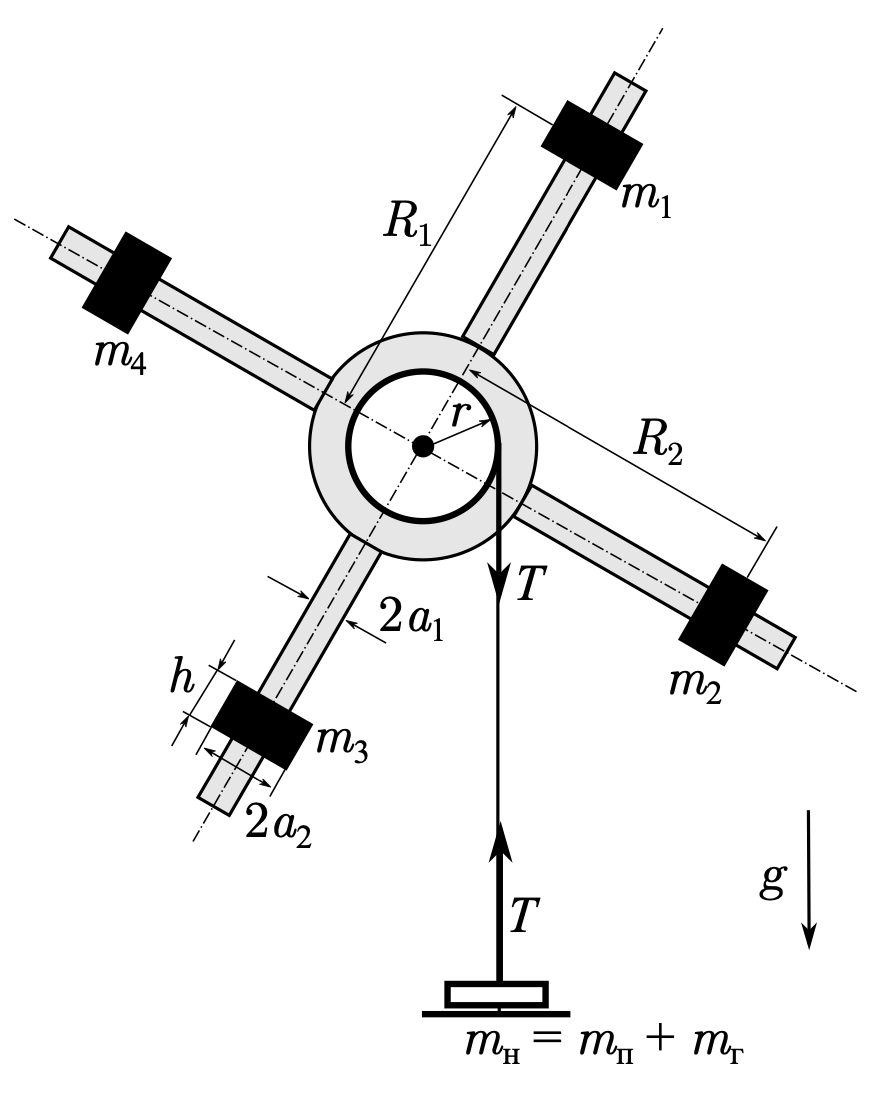
\includegraphics[width=0.47\linewidth,center]{p1.png}
    \caption{Крестообразный маятник Обербека}
    \label{fig:my_label}
\end{figure}

\textbf{Экспериментальная установка.}Для экспериментального исследования закона вращательного движения (1) в работе используется крестообразный «маятник», устройство которого изображено на рис. 1.
Маятник состоит из четырех тонких стержней радиуса $a$, укрепленных
на втулке под прямым углом друг к другу. Втулка и два шкива различных радиусов ($r_1$ и $r_2$) насажены на общую ось. Ось закреплена в подшипниках, так что вся система может свободно вращаться вокруг горизонтальной оси. Момент инерции $I$ маятника можно изменять, передвигая грузы $m_i$ ($i = 1\dots4$) вдоль стержней и меняя $R_i$. На один из шкивов маятника навита тонкая нить. Привязанная к ней легкая платформа известной массы $m_\text{п}$, служит для размещения перегрузков $m_\text{г}$.

Установка оснащена датчиком, позволяющим фиксировать моменты времени прохождения концов стержней через него. Данные с датчика передаются на компьютер для последующей обработки и получения
зависимостей угла поворота $\varphi(t)$, угловой скорости $\omega \equiv \dot{\varphi}$ и углового ускорения маятника $\beta \equiv \ddot{\varphi}$ от времени, а также углового ускорения от
угловой скорости $\beta (\omega)$.

\textbf{Вывод уравнения движения маятника.} Рассмотрим силы, действующие на маятник. Основной вращающий момент создаётся подвешенным на нити перегрузком. Непосредственно на маятник действует момент силы натяжения нити: $M_\text{н} = rT$, где $r$ - радиус шкива ($r_1$ или $r_2$). Силу $T$ выразим из уравнения движения платформы:
$m_\text{н} \ddot y = m_\text{н}g - T$, где $m_\text{н} = m_\text{п} + m_\text{г}$, — масса платформы с перегрузком.
Ускорение платформы связано с угловым ускорением маятника условием нерастяжимости нити $\ddot y = \beta r$. Отсюда момент силы натяжения нити
\begin{equation}
    M_\text{н} = m_\text{н}r\left(g - \beta r\right).
\end{equation}
Вращению маятника препятствует момент силы трения в оси $M_\text{тр}$. Таким образом, с учетом (2) уравнение (1) может быть записано как
\begin{equation}
    \left(I + m_\text{н}r^2\right)\beta = m_\text{н}gr - M_\text{тр}.
\end{equation}
Заметим, что в наших опытах, как правило, $m_\text{н}r^2 \ll I$, и соответственно $M_\text{н} \approx m_\text{н}gr$. Если трение мало, $M_\text{тр} \ll m_\text{н}gr$, то маятник будет раскручиваться с постоянным угловым ускорением $\beta_0 \approx m_\text{н}gr / I$.

Поскольку зависимость момента силы трения от нагрузки на маятник и скорости его вращения не известна (её исследование -- отдельная экспериментальная задача), методика измерения должна быть построена так, чтобы минимизировать или вовсе исключить влияние $M_\text{тр}$. Можно высказать следующие качественные соображения о природе и величине $M_\text{тр}$. Она может иметь как составляющую, пропорциональную силе реакции в оси $N$ (сухое трение в подшипниках), так и составляющую, пропорциональную угловой скорости и вращения маятника (вязкое трение в подшипниках и сопротивление воздуха).
Учитывая, что сила реакции уравновешеннего маятника равна
$N = m_\text{м}g + T$, где $m_\text{м}$ масса маятника (как правило, $m_\text{м} \gg m_\text{н}$), можно записать
\begin{equation}
    M_\text{тр} \simeq \left(1 + \frac{m_\text{н}}{m_\text{м}}\right) M_0 + \eta \omega \approx M_0 + \eta \omega,
\end{equation}
где $M_0$ — момент сил трения для покоящегося маятника при нулевой массе подвеса (минимальное значение силы трения), $\eta$ - некоторый коэффициент, отвечающий за вязкое трение.

\textbf{Методика эксперимента.} Малость величины трения $M_\text{тр}$ в работе обеспечивается за счёт использования в креплении подшипников качения. Однако учёт трения всё же оказывается необходим, поскольку оно существенно влияет на результаты опыта как при малых массах перегрузков (когда $m_\text{н} \thicksim  M_0/gr$), так и при больших, поскольку при увеличении $m_\text{н}$ возрастает сила реакции в оси и угловая скорость вра-щения маятника, а с ней и вязкое трение.

Влияние вязкой составляющей трения можно исключить следующим образом. Экспериментальная установка позволяет измерять зависимость углового ускорения от угловой скорости $\beta(\omega)$. Если верны высказанные выше соображения о величине силы трения, из (3) и (4) следует, что угловое ускорение должно быть линейной функцией угловой скорости: $\beta = \beta_0 + k\omega$. В таком случае, определив по экспериментальным данным (с помощью расчётной программы) коэффициенты прямой, можно найти начальное угловое ускорение $\beta_0$, значение которого и используется при проверке основного соотношения (3) при различных параметрах системы ($m_\text{н}$, $I$, $r$).

Момент инерции всей системы вычисляется по теореме Гюйгенса- Штейнера:
\begin{equation}
    I = I_0 + \sum_{i = 1}^{4}\left(I_i + m_i R_i^2\right),
\end{equation}
где $I_0$ - момент инерции системы без грузов, $I_i$  -- момент инерции $i$-го груза относительно оси, проходящей через его
центр масс (перпендикулярно плоскости рис. 1).
